\section{DESIGN RATIONALE}
\label{app:rationale}
\readorder{20}

This appendix carries the parts of the arguments of \cref{sec:method} that the main text only summarises. Some subsections, among them \cref{app:mirror,app:qw}, restate the main text's step before completing it.

\subsection{The Mirror Attractor}
\label{app:mirror}

The attention layer of \cref{eq:context-gat} computes logits $e_{ij} = \mathbf{a}^\top \mathrm{LeakyReLU}(\mathbf{W}_{\mathrm{dst}} \mathbf{h}_i + \mathbf{W}_{\mathrm{src}} \mathbf{h}_j)$ and aggregates $\sum_j \att_{ij} \mathbf{W}_{\mathrm{src}}\mathbf{h}_j$, so the destination feature $\mathbf{h}_i$ enters the \emph{attention} but never the \emph{value} \citep{brody2022}. With $\vz_i$ as the destination feature, the selection channel of \cref{sec:inference} opens. What the type query gives up is state-specific attention, which belongs in the decoder (as type-dependent loadings or a low-rank interaction with $\vz$) rather than in the context encoder.

\flag{MERGE}{repeats 2.3 and 2.7; keep the attention derivation above} The diagnostic is the within-type coefficient of determination of $\vz_i$ regressed on $\vc_i$ against a within-type permuted control (\cref{sec:selection}). The correlation between $\att_{ij}$ and $\simop(\vz_i,\vz_j)$ would serve under a $\vz$ query; with the type as query and types as sources the attention weights depend on the types alone (\cref{eq:context-closed}), and the correlation is vacuous. Downstream, a mirror is indistinguishable from ordinary posterior collapse of $\vw$; a free-bits remedy \citep{kingma2016} would mask it and leave the divergence uninterpretable, which is why the mirror is ruled out first.

Zeroing $\vz_i$ while keeping self-loops is not an alternative: the softmax still spends attention mass on the self-edge, down-weighting neighbours, and under $\vz \sim \N(\mathbf{0},\vI)$ the origin is the prior mean, so a zero vector asserts ``this cell is average'' rather than ``ignore this cell''.

\subsection{Why the Context Gets No Per-Edge Geometry, and Why the Graph Is Delaunay}
\label{app:graph}

\flag{TRIM}{four floats for one design choice; keep tab:contact and one figure} A discretised contact indicator (touching, near, far) looks as if it dodges the collinearity objection of \cref{sec:inference}, but on this platform, whose segmented polygons rarely touch, whether two of them touch is largely a measurement of local density: dense regions touch, sparse regions do not. The indicator would smuggle density back in, in the confounded direction, and a tolerance parameter only moves the threshold. \Cref{fig:graph-compare} shows it on one field: exact contact leaves most cells without a neighbour, a $1\um$ tolerance connects the dense tissue but leaves the separated cells of the sparse tissue isolated, and Delaunay adjacency connects them all.

\begin{figure}[t]
\centering
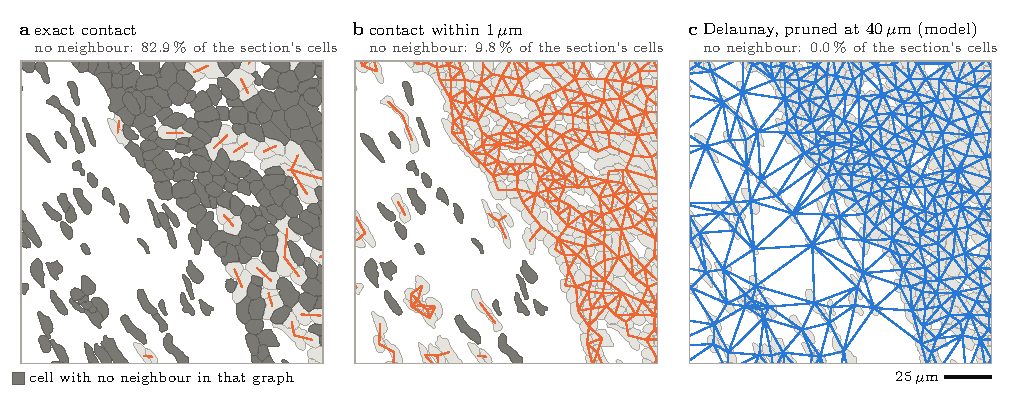
\includegraphics[width=\textwidth]{figures/fig_graph_compare}
\caption{Three neighbour graphs on one $160\um$ field of the primary section, each a subset of the model's edge set. \textbf{a},~Edges whose segmented polygons touch. \textbf{b},~Edges along which the two polygons run within $1\um$ of each other, the contact of \cref{tab:contact}. \textbf{c},~The model's graph: Delaunay adjacency pruned at $40\um$. Cells with no edge in a panel's graph are dark. The share above each panel is over the whole section, among cells with at least one edge in~c. The field is chosen to be representative: among fields that contain both sparse and dense tissue, it is the one whose shares under a and b are closest to the section's. Edges are drawn at one width; their weights in $\beta$ are illustrated in \cref{fig:overview}a. All panels share one scale.}
\label{fig:graph-compare}
\end{figure}

Delaunay adjacency resolves it: two cells are neighbours if and only if their Voronoi cells share a face, which is the correct notion of adjacency for a packing, built from centroids alone. The one parameter that returns is the pruning of long edges, and it is much less sensitive than choosing a neighbour count. The Voronoi face length is used in the kernel rather than shared segmented boundary because the Voronoi face is where the boundary between two cells effectively lies, its length is a contact-extent proxy defined whether or not the polygons touch, and it is independent of the expansion setting (\cref{fig:voronoi-face}).

\begin{figure}[t]
\centering
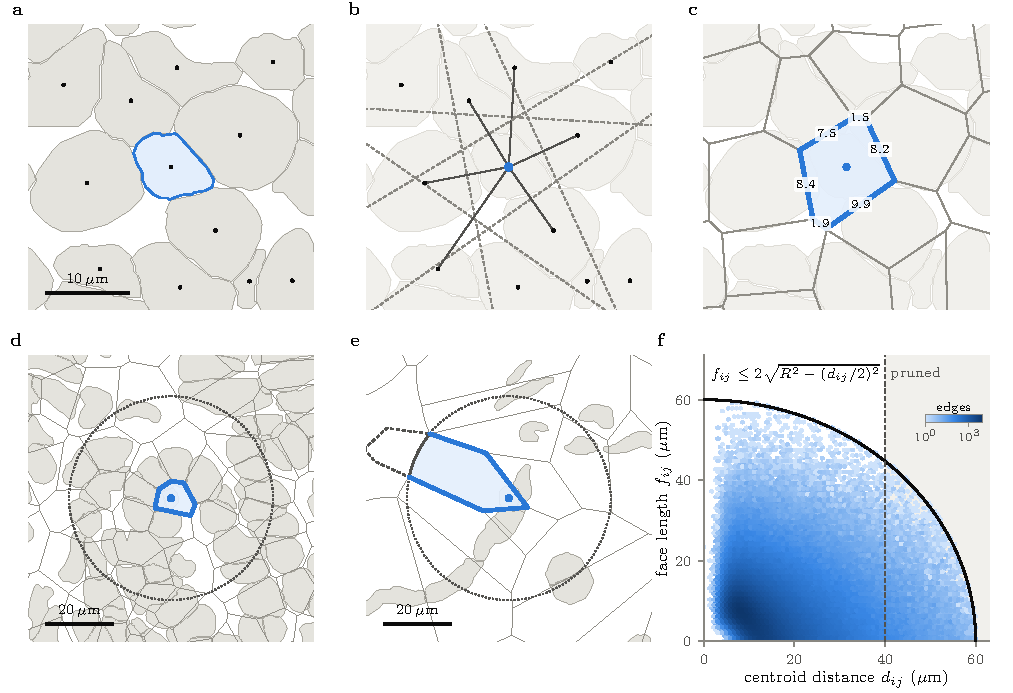
\includegraphics[width=\textwidth]{figures/fig_voronoi_face}
\caption{How the Voronoi face is built, and what bounds it, on the primary section. \textbf{a},~Segmented polygons and their centroids around a typical cell (blue). \textbf{b},~The polygons are set aside; each neighbour contributes the perpendicular bisector (dashed) of the segment joining the two centroids. \textbf{c},~The bisectors cut one another, and what survives between the cell and a neighbour is the face $f_{ij}$ (blue, length in $\mu$m); the shaded area is the cell's Voronoi region. Panels a--c share one scale. \textbf{d},~A dense neighbourhood and \textbf{e},~a cell at a tissue border, at one scale, each with the $30\um$ clip disc (dotted). At the border the unclipped region (dashed) runs into the gap, the disc bounds it, and the dark stretch of the outline between two faces is the clip arc. \textbf{f},~Face length against centroid distance for every edge of the section. Clipping bounds each face by the chord $2\sqrt{R^2-(d_{ij}/2)^2}$ of the disc, with $R = 30\um$, and removes every edge with $d_{ij} \ge 2R$; the model keeps edges up to $40\um$ (unshaded).}
\label{fig:voronoi-face}
\end{figure}

\Cref{tab:contact} and \cref{fig:contact-kernel} make the comparison concrete on every section. The sections were segmented mostly by an interior RNA stain rather than by nuclear expansion, and adjacent polygons still rarely touch. A contact kernel is therefore zero on about half of the edges, and it leaves a density-dependent share of cells with no leakage at all: up to a third of cells in the sparsest fifth of a section, almost none in the densest. Whether a cell can receive leakage would then be decided by local density, which is part of the niche. The Voronoi kernel gives every connected cell the same leak budget $\kappa$. Both kernels give nearer neighbours more weight; for $\beta$ that dependence is the one the distance decay introduces by design, and the face does not add to it.

\begin{table}[t]
\centering
\caption{Segmented-polygon contact as a leakage kernel, against the Voronoi-face kernel $\beta$, on every section and on the model's edge set (Delaunay adjacency pruned at $40\um$). Both kernels use the same distance decay $\exp(-d_{ij}/\tau)$ and the same row normalisation. The contact kernel weights an edge by the length of membrane along which the two segmented polygons run within $1\um$ of each other; $\beta$ weights it by the Voronoi face. FF: fresh frozen. \emph{Touching}: adjacent pairs whose polygons are at zero distance. \emph{No-leak cells}: connected cells whose kernel row is all zero, so that they receive no leakage at any $\kappa$; \emph{sparse} and \emph{dense} are the lowest and highest fifth of cells by the number of centroids within $20\um$. $\rho$: Spearman correlation, over edges, between a neighbour's share of the row and the gap between the two polygons. The Voronoi kernel has no zero-weight edges and no no-leak cells on any section. Its dependence on the gap is that of the distance decay alone (shares from the decay alone: $\rho$ between $-0.49$ and $-0.62$).}
\label{tab:contact}
\small
\setlength{\tabcolsep}{3.5pt}
\begin{tabular}{@{}lrrrrrrrrrr@{}}
\toprule
& \multicolumn{3}{c}{Segmented by (\% cells)} & \multicolumn{2}{c}{Edges (\%)} & \multicolumn{3}{c}{No-leak cells, contact (\%)} & \multicolumn{2}{c}{$\rho$(share, gap)} \\
\cmidrule(lr){2-4}\cmidrule(lr){5-6}\cmidrule(lr){7-9}\cmidrule(l){10-11}
Section & interior & boundary & nucleus & touching & no contact & all & sparse & dense & contact & $\beta$ \\
\midrule
Ovarian cancer (FFPE) & 69 & 29 & 2.0 & 3.5 & 47 & 9.8 & 33.6 & 0.6 & $-0.82$ & $-0.48$ \\
Lung cancer (FFPE) & 82 & 16 & 2.2 & 2.7 & 57 & 11.1 & 27.4 & 0.7 & $-0.84$ & $-0.55$ \\
Ovarian cancer (FF) & 70 & 28 & 2.5 & 6.7 & 38 & 3.2 & 10.6 & 0.1 & $-0.80$ & $-0.52$ \\
Lung TMA, section A & 87 & 12 & 1.0 & 2.2 & 47 & 6.3 & 24.8 & 0.1 & $-0.84$ & $-0.54$ \\
Lung TMA, section B & 87 & 12 & 1.2 & 2.2 & 47 & 6.2 & 24.6 & 0.1 & $-0.84$ & $-0.53$ \\
\bottomrule
\end{tabular}
\end{table}

\begin{figure}[t]
\centering
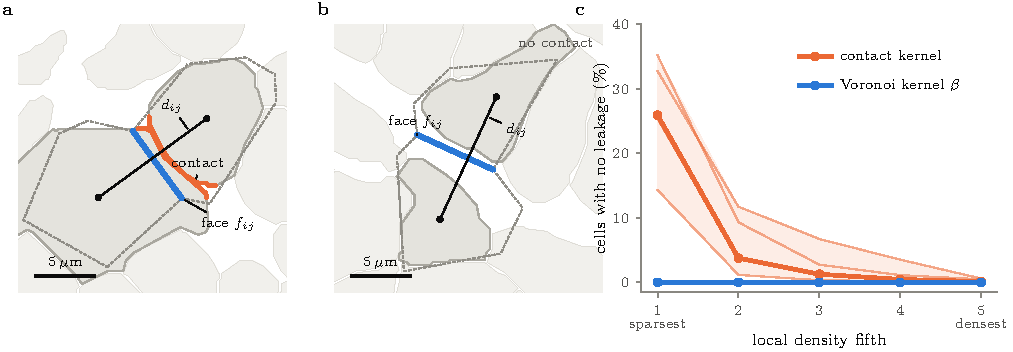
\includegraphics[width=\textwidth]{figures/fig_contact_kernel}
\caption{Why the leakage kernel is built on Voronoi faces rather than on segmented contact. \textbf{a},~An edge whose segmented polygons touch and \textbf{b},~an edge whose polygons do not, each the edge of its kind closest to the primary section's median centroid distance and median face length. The two have almost the same centroid distance $d_{ij}$ and face $f_{ij}$ (blue), which is all the kernel $\beta$ uses; contact (orange), the stretch of each cell's membrane within $1\um$ of the other cell, is present in a and absent in b. Dashed lines are the two cells' Voronoi regions; both panels share one scale. \textbf{c},~The share of cells that a contact-weighted kernel would leave with no leakage at all, by fifth of local density (centroids within $20\um$), on each section of \cref{tab:contact}: the median (bold), the range (band) and each section (thin). Both kernels use the model's edge set, the same distance decay and the same row normalisation; the Voronoi kernel leaves no connected cell without leakage on any section.}
\label{fig:contact-kernel}
\end{figure}


\flag{TRIM}{attention-sink test is development history, also in tab:deviations2; keep one} One consequence of the softmax over a Delaunay neighbourhood should be stated. With the type as query and one-hot types as sources, the logit of edge $ij$ depends on $(t_i, t_j)$ alone, say $s_{t_i t_j}$, and grouping the neighbours by type gives, per head,
\begin{equation}
  \mathbf{g}_i = \frac{\sum_k y_{ik}\, e^{s_{t_i k}}\, \mathbf{W}_{\mathrm{src}}\mathbf{e}_k}{\sum_k y_{ik}\, e^{s_{t_i k}}},
  \label{eq:context-closed}
\end{equation}
with $\mathbf{e}_k$ the $k$-th unit vector: a learned, type-specific reweighting of the neighbour composition in which the degree cancels. The context therefore depends on the fractions $\vy_i$, not on the counts. It distinguishes one tumour neighbour among six from five among six, but not a neighbourhood from the same neighbourhood with every type count scaled up together; in particular a single-type neighbourhood gives the same context whatever its size. On this tessellation the degree is nearly constant across the section, so a fraction determines a count and the blindness costs little. An attention sink, a fixed null logit that joins every softmax and restores a saturating dependence on the count, is implemented and was tested over three seeds. It learned no dose response, placing its half-point below a single neighbour, did not improve the held-out transport of the response, and in two of the seeds made the prior mean read the context less faithfully. It is therefore left off. It would become meaningful only on a graph whose degree varies, where the invariance target would have to grow with it.

\flag{CUT}{the edge-feature run was never done; cut, or run it and report} The fallback is empirical. If $\mpsi$ predicts responses poorly, or held-out reconstruction is worse than a comparison run whose attention layer carries edge features (distance, face length), that is direct evidence that the continuous signal mattered. If it is added back, the correlation between $\att_{ij}$ and $\beta_{ij}$ must be monitored: a high correlation means the attention has rediscovered the leakage kernel and $\vw$ is becoming collinear with $\rhobar$. That risk is tolerable while $\kappa$ is fixed, since there is no free contamination parameter to feed, and intolerable once $\kappa$ is estimated. \pending{the edge-feature comparison run has not been performed}

\subsection{The Image Descriptor and Its Mask}
\label{app:image}

\flag{TRIM}{the KRONOS vs KRONOS2 comparison can shrink to one sentence} The image descriptor $\vPhi_i$ is the embedding of a $128\um$ field around the cell ($256$ pixels at $0.5\um$ per pixel) in the section's four morphology channels (\cref{fig:overview}b), by KRONOS, a frozen foundation model for multiplexed tissue images \citep{kronos2025}: its first release, a ViT-S/16 with a $384$-dimensional embedding. The channels map onto the model's marker vocabulary only approximately: the membrane and $\alpha$SMA channels are antibody mixes read as their named component, and 18S RNA lies outside the vocabulary and is given an unused marker identity. The cell is removed by setting a disc around it to zero, not its own polygon: a polygon-shaped hole would keep the cell's outline, the most type-informative feature of all. The disc is centred on the crop anchor and has one radius for every cell, so the hole carries no information about the cell it removes, and it is filled with zeros, a constant artefact that the image model encodes identically for every cell. Its radius is the smallest that covers essentially every cell (\cref{fig:mask-radius}). A cell's covering radius, the radius of the smallest disc centred on its anchor that contains its polygon, has a long tail of elongated smooth-muscle cells; a $25\um$ disc leaves six cells of the primary section outside it and masks $12\%$ of the field. Those six cells were left out of the comparison below, and in the model their image descriptor is set to zero. A cell that sticks out of the disc would leak the identity the disc exists to remove, so partial coverage is not an option. At this density the disc also removes the cell's first ring or two, so $\vPhi_i$ describes the tissue beyond roughly $25\um$.

\begin{figure}[t]
\centering
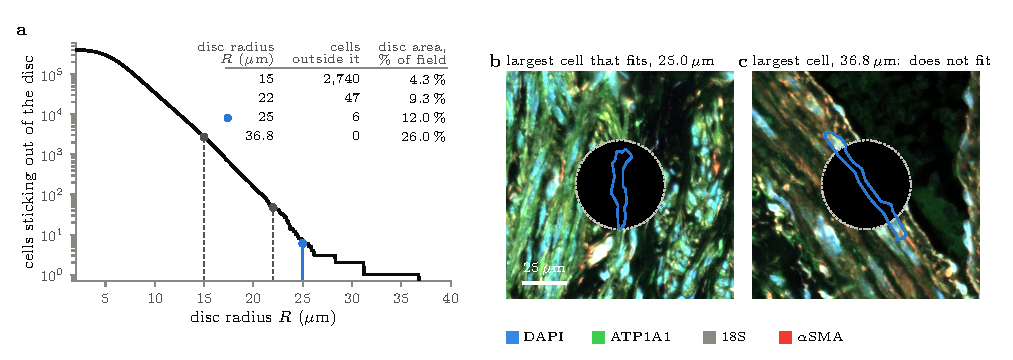
\includegraphics[width=\textwidth]{figures/fig_mask_radius}
\caption{Why the mask is a $25\um$ disc, on the primary section. \textbf{a},~The number of cells that would stick out of a disc of radius $R$ centred on the crop anchor, from each cell's covering radius; the table gives the radii considered, the cells left outside, and the share of the $128\um$ field each disc masks. The last row is the largest cell on the section. \textbf{b},~The largest cell that fits the chosen disc and \textbf{c},~the largest cell on the section, which does not, both drawn as the image model receives them: four channels, disc set to zero, with the cell's outline for reference. Both are elongated smooth-muscle cells.}
\label{fig:mask-radius}
\end{figure}

\Cref{tab:masking} shows what each mask leaves in the embedding, read by a multinomial logistic regression that predicts the cell's lineage label from it. The split is spatial, in tiles with a margin, because the fields of neighbouring cells overlap almost completely and a random split would put the same pixels on both sides. Three readings follow. The cell alone carries more type information than the whole patch: the surrounding tissue dilutes it rather than adding to it. Removing the cell costs little, because the patch embedding is dominated by its surroundings (\cref{fig:kronos-umap}a,~b). And the masked patch predicts the label less well than the neighbours' labels alone, so what it knows about the cell is what type-homogeneous neighbourhoods imply, which is what a descriptor of the niche should carry. On the masked patch the first release does at least as well as its successor KRONOS2 (a ViT-B/16 with a $768$-dimensional embedding, from the same authors); KRONOS2 is better only on the cell alone, where the model deliberately does not look. We therefore use the first release: its embedding is half as wide ($384$ against $768$ dimensions), which keeps the image part of the context descriptor small, and it embeds cells about five times faster.

\begin{table}[t]
\centering
\caption{What each mask leaves in the image embedding, on the primary section: macro one-versus-rest AUC of a multinomial logistic regression predicting the cell's lineage label (the labels the model is fitted with; 11 classes, Unassigned cells excluded as targets but counted as neighbours) from the embedding, on a spatial split ($1\,$mm tiles, cells within half a field of a tile edge dropped; $40{,}000$ training and about $74{,}000$ test cells), for the two releases of the image model, KRONOS and KRONOS2 \citep{kronos2025}. The first row predicts the label from the neighbours' labels alone, with no image. The model uses KRONOS with the disc zeroed (bold).}
\label{tab:masking}
\small
\begin{tabular}{@{}lcc@{}}
\toprule
Input to the classifier & KRONOS & KRONOS2 \\
\midrule
Neighbours' labels, no image & \multicolumn{2}{c}{$0.918$} \\
Whole patch & $0.881$ & $0.878$ \\
Disc over the cell zeroed & $\mathbf{0.857}$ & $0.846$ \\
The cell alone & $0.905$ & $0.919$ \\
The cell alone, native resolution & $0.923$ & -- \\
\bottomrule
\end{tabular}
\end{table}

\begin{figure}[t]
\centering
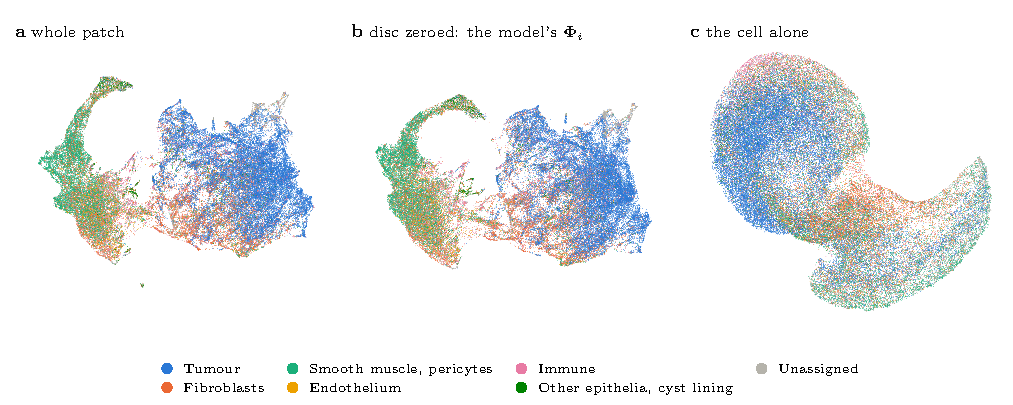
\includegraphics[width=\textwidth]{figures/fig_kronos_umap}
\caption{\flag{CUT}{adds little beyond tab:masking} The KRONOS embedding (first release, the one the model uses) under three masks, as UMAPs of the same $60{,}000$ cells of the primary section (principal components, then UMAP). \textbf{a},~The whole $128\um$ patch. \textbf{b},~The disc over the cell zeroed, the descriptor $\vPhi_i$ the model uses; it differs little from~a, because the patch is dominated by the surrounding tissue. \textbf{c},~Everything outside the cell's polygon zeroed, what the cell alone carries. Colour is the section's lineage label, the one the model is fitted with, with the smaller lineages grouped for display. Unassigned includes a low-depth class of mixed lineage that the section's original annotation had called a tumour subtype.}
\label{fig:kronos-umap}
\end{figure}

\subsection{Three Routes to a Vanishing Response Divergence}
\label{app:qw}

\flag{MERGE}{table repeats diagnostic (ii) of 2.7; fold into that sentence} \begin{center}
\begin{tabular}{@{}>{\raggedright\arraybackslash}p{0.2\textwidth}>{\raggedright\arraybackslash}p{0.4\textwidth}>{\raggedright\arraybackslash}p{0.34\textwidth}@{}}
\toprule
Cause & Check & Fix \\
\midrule
Posterior collapse & $\alphaw$ large relative to reconstruction & lower $\alphaw$; free bits \\
Mirror & within-type $R^2$ of $\vz_i$ on $\vc_i$ vs.\ permuted control & type embedding as query; types only as sources \\
Starved of ego evidence & does the response posterior receive $\vx_i$ directly? & add the direct path \\
\bottomrule
\end{tabular}
\end{center}

\subsection{Conditional Invariance and Label Granularity}
\label{app:conditional}

\flag{CHECK}{todo still open: the numbers are in DisCoVR's Table 19 (checked 09-23) but not quoted in the manuscript or devlog, so this needs a read of that table; the four-reasons list overlaps 2.1 and 2.5} The marginal-invariance failure is documented by \citet{slavutsky2025} for the conditional subspace VAE \citep{klys2018}, whose invariance drives the agreement between the shared code and the nuisance variable to zero while collapsing its agreement with cell type \todo{quote the exact numbers from that comparison}. Lineage-level labels are preferable to finer or state-defined ones for four reasons: fine labels leave $\vz$ with nothing to carry, they block more of the position$\to$fate$\to$expression path, they destroy the overlap that any conditional comparison needs, and, because $t_i$ is itself a function of $\vx_i$, hence of leakage and of any response that moves a cell across a label boundary, conditioning on it conditions on a descendant of the niche, so that even the true intrinsic state can depend on $\vy_i$ given $t_i$ near label boundaries \citep{hernan2004}.

\subsection{The Leak Fraction: Grid Range and Upgrade Path}
\label{app:kappa}

The grid runs from zero, the nested no-correction null, to $0.4$. On this platform a typical cell carries misassigned transcripts of about a tenth of its counts, and heavily contaminated cells are rare \citep{yang2025mistic}. The operating point $\kappa = 0.1$ (\cref{sec:setup}) matches that typical value, and the top of the grid is deliberately conservative, several times it.

This version of the model sweeps $\kappa$; it cannot estimate it. Assigning transcripts to cells by position does not settle it either: counts of transcripts that lie nearer a neighbour's nucleus than the cell's own are dominated by segmentation geometry, since a large cell beside small ones counts its own far-side transcripts as foreign, so such counts bound leakage from above but do not identify how it scales with the depth of the receiving or the donating cell. Estimation needs two views of one cell that share a foreign profile at different contamination levels, which a nuclear/extranuclear split of the transcript coordinates provides. Its identifying condition is that gene-wise nuclear retention varies across genes, which is also a reason to expect the gene-specific leakage that the main model does not represent (\cref{sec:generative}), and which a two-view likelihood would be the natural place to model; with constant retention both views lie on the same line between $\vrho_i$ and $\rhobar_i$ and nothing is pinned. Adding it does not restructure the model: the likelihood becomes a multinomial over $2G$ bins and $\kappa$ moves from hyperparameter to latent. We leave it as future work.

What the data say about $\kappa$ can be stated exactly at the level of compositions.

\Cref{prop:kappa-bound} (\cref{sec:sweep}) states it; the proof follows.
\begin{proof}[Proof of \cref{prop:kappa-bound}]
The clean composition implied by $\kappa'$ is $\vrho_i(\kappa') = (\vp_i - \kappa'\rhobar_i)/(1-\kappa')$, which sums to one for every $\kappa'$ and is non-negative in gene $g$ if and only if $\kappa'\bar\rho_{ig} \le p_{ig}$; this holds for every gene if and only if $\kappa' \le \bar\kappa_i$. Since $p_{ig}/\bar\rho_{ig} = \kappa + (1-\kappa)\rho_{ig}/\bar\rho_{ig} \ge \kappa$, the true value lies below the bound, and meets it exactly when a gene the neighbours express has zero share in the cell's own composition.
\end{proof}

The data therefore bound $\kappa$ from above and never from below, and a section-wide $\kappa$ must respect the bound of every cell. They pin it only through a gene the cell cannot express itself, such as a marker that an external atlas excludes for the cell's type, or through a second view of the cell such as a nuclear/extranuclear split. \Cref{fig:kappa-bound} draws both cases. The statement is about compositions: with counts the bound is soft, since a $\kappa$ above it charges each cell for neighbour transcripts it does not show, and the decoder's form can narrow the interval further, which is the route that expected low-dimensionality takes and that a response to the niche weakens (\cref{sec:intro}).

\begin{figure}[t]
\centering
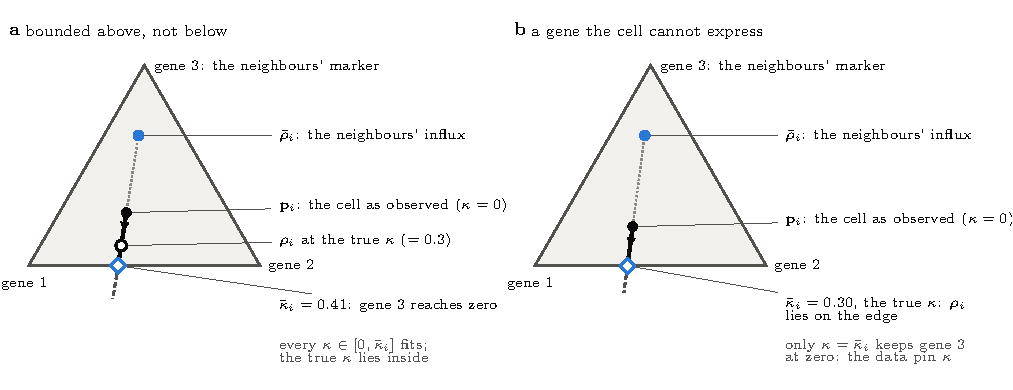
\includegraphics[width=\textwidth]{figures/fig_kappa_bound}
\caption{What the data say about $\kappa$, on the simplex of three genes; schematic, with compositions chosen for legibility. With the neighbours' influx $\rhobar_i$ held fixed, each $\kappa$ implies the clean composition $\vrho_i(\kappa) = (\vp_i - \kappa\rhobar_i)/(1-\kappa)$: a line that starts at the observed composition $\vp_i$ ($\kappa = 0$) and runs away from $\rhobar_i$ (arrow). It is valid until it leaves the simplex at $\bar\kappa_i$ (diamond) and invalid beyond (dashed). \textbf{a},~A cell that expresses a little of the neighbours' marker itself: every $\kappa \in [0, \bar\kappa_i]$ reproduces $\vp_i$ exactly, and the true value lies inside. \textbf{b},~A cell that cannot express the marker: its true composition lies on the edge, the line leaves the simplex exactly there, and $\bar\kappa_i$ is the true $\kappa$.}
\label{fig:kappa-bound}
\end{figure}

\flag{TRIM}{repeats def:breakdown and the fig:breakdown caption; keep the fibroblast example} \Cref{def:breakdown} is easiest to read on an example. A readout is any number reported from a fit, for instance how much a fibroblast programme differs between fibroblasts next to tumour and fibroblasts in stroma. At $\kappa = 0$ the model assigns all of that difference to the cells themselves. Refitting at each larger $\kappa$ attributes more of the resemblance between neighbours to leakage, so a difference that is only leakage shrinks toward its null value, and one that reflects biology persists. The breakdown point $\kappa^\star$ is the smallest leak fraction at which the readout can no longer be told from its null, or changes sign: how much leakage it would take to explain the readout away. \Cref{fig:breakdown} shows the four cases. A readout that survives every grid value cannot be explained by leakage of the modelled form up to the top of the grid (a). A contrast may shrink as $\kappa$ grows without breaking down (b): readouts shrink by construction, because the mixture takes over part of the resemblance between neighbours, and the contrast stands as long as its interval stays clear of zero. A readout that breaks down inside the grid is explained away by that much leakage (c), and one that breaks down at the first grid point above zero is explained away by any leakage at all (d). The higher the breakdown point, the stronger the finding. Read with \cref{fig:kappa-bound}, the two say what a finding would need: the data bound the leak fraction from above, so a readout whose breakdown point lay above that bound would survive every leak fraction the data allow. That bound is not computed on the sections here (\cref{prop:kappa-bound}), so what the grid supports is the weaker statement that a readout surviving it survives every leak fraction up to $0.4$.

\begin{figure}[t]
\centering
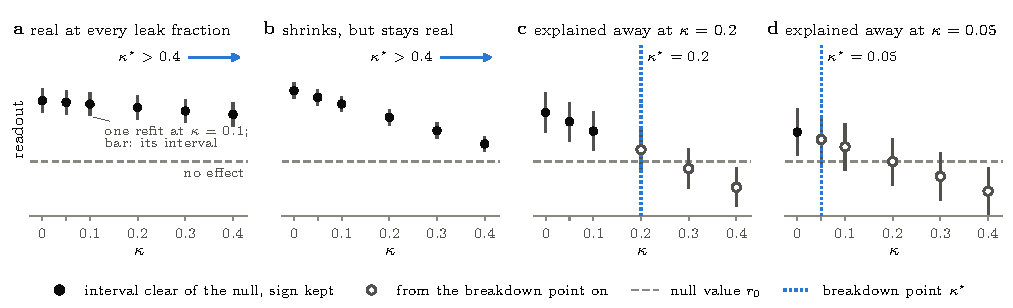
\includegraphics[width=\textwidth]{figures/fig_breakdown}
\caption{The breakdown point of \cref{def:breakdown}, on four schematic readouts: four different candidate findings, not four ways of choosing $\kappa$, which is never chosen. The curves are illustrative, not fitted, and only the grid of $\kappa$ is the model's. Each panel shows a readout at every grid value with its interval (bars) and its null value $r_0$ (dashed). Filled markers: the interval is clear of the null and the readout keeps the sign it has at $\kappa = 0$; hollow markers: from the breakdown point $\kappa^\star$ (dotted) on. Each point is a separate fit at that $\kappa$. \textbf{a},~A signed contrast that survives the grid, reported as $\kappa^\star > 0.4$. \textbf{b},~A contrast that shrinks as $\kappa$ grows, as expected by construction because more of the resemblance between neighbours is assigned to the mixture, but stays clear of zero: it also survives. \textbf{c},~A contrast that $20\%$ leakage explains away, $\kappa^\star = 0.2$; its sign flips beyond it. \textbf{d},~A contrast that breaks down at the first grid point above zero, $\kappa^\star = 0.05$: any leakage explains it away, so it is not separable from leakage of the modelled form.}
\label{fig:breakdown}
\end{figure}

\subsection{Learned Variances: What to Learn and What Not To}
\label{app:variances}

If a conditional $\sigma_w(\vc, t)$ is wanted, because it would standardise deviation against local variability so that a deviation of two in a niche where everyone deviates by two does not read as anomalous, it must be bounded, e.g.\ $\sigma_w \in [0.5, 2]$ through a scaled sigmoid, so that it cannot inflate away, and its mean over cells must be checked for upward drift over training.

The prior on $\vz$ is a standard normal. A richer prior, a mixture with one component per type or a VampPrior with archetypal pseudo-inputs \citep{tomczak2018}, would be a genuine upgrade for cell-type structure and would make $t$ a latent rather than an input, but that is a different change, not a variance question.
